\documentclass{article}
\iffalse
This file is protected by Copyright. Please refer to the COPYRIGHT file
distributed with this source distribution.

This file is part of OpenCPI <http://www.opencpi.org>

OpenCPI is free software: you can redistribute it and/or modify it under the
terms of the GNU Lesser General Public License as published by the Free Software
Foundation, either version 3 of the License, or (at your option) any later
version.

OpenCPI is distributed in the hope that it will be useful, but WITHOUT ANY
WARRANTY; without even the implied warranty of MERCHANTABILITY or FITNESS FOR A
PARTICULAR PURPOSE. See the GNU Lesser General Public License for more details.

You should have received a copy of the GNU Lesser General Public License along
with this program. If not, see <http://www.gnu.org/licenses/>.
\fi

\author{} % Force author to be blank
%----------------------------------------------------------------------------------------
% Paper size, orientation and margins
%----------------------------------------------------------------------------------------
\usepackage{geometry}
\geometry{
	letterpaper,			% paper type
	portrait,				% text direction
	left=.75in,				% left margin
	top=.75in,				% top margin
	right=.75in,			% right margin
	bottom=.75in			% bottom margin
 }
%----------------------------------------------------------------------------------------
% Header/Footer
%----------------------------------------------------------------------------------------
\usepackage{fancyhdr} \pagestyle{fancy} % required for fancy headers
\renewcommand{\headrulewidth}{0.5pt}
\renewcommand{\footrulewidth}{0.5pt}
\newcommand{\terminaloutput}[1]{\texttt{#1}}
\rhead{\small{ANGRYVIPER Team}}
%----------------------------------------------------------------------------------------
% Appendix packages
%----------------------------------------------------------------------------------------
\usepackage[toc,page]{appendix}
%----------------------------------------------------------------------------------------
% Defined Commands & Renamed Commands
%----------------------------------------------------------------------------------------
\renewcommand{\contentsname}{Table of Contents}
\renewcommand{\listfigurename}{List of Figures}
\renewcommand{\listtablename}{List of Tables}
\newcommand{\todo}[1]{\textcolor{red}{TODO: #1}\PackageWarning{TODO:}{#1}} % To do notes
\newcommand{\code}[1]{\texttt{#1}} % For inline code snippet or command line
%----------------------------------------------------------------------------------------
% Various pacakges
%----------------------------------------------------------------------------------------
\usepackage{hyperref} % for linking urls and lists
\usepackage{graphicx} % for including pictures by file
\usepackage{listings} % for coding language styles
\usepackage{rotating} % for sideways table
\usepackage{pifont}   % for sideways table
\usepackage{pdflscape} % for landscape view
\usepackage{scrextend}
%----------------------------------------------------------------------------------------
% Table packages
%----------------------------------------------------------------------------------------
\usepackage{tabularx} % c=center,l=left,r=right,X=fill
\usepackage{float}
\floatstyle{plaintop}
\usepackage[tableposition=top]{caption}
\newcolumntype{P}[1]{>{\centering\arraybackslash}p{#1}}
\newcolumntype{M}[1]{>{\centering\arraybackslash}m{#1}}
%----------------------------------------------------------------------------------------
% Block Diagram / FSM Drawings
%----------------------------------------------------------------------------------------
\usepackage{tikz}
\usetikzlibrary{shapes,arrows,fit,positioning}
\usetikzlibrary{automata} % used for the fsm
\usetikzlibrary{calc} % For duplicating clients
\usepgfmodule{oo} % To define a client box
%----------------------------------------------------------------------------------------
% Colors Used
%----------------------------------------------------------------------------------------
\usepackage{colortbl}
\definecolor{blue}{rgb}{.7,.8,.9}
\definecolor{ceruleanblue}{rgb}{0.16, 0.32, 0.75}
\definecolor{drkgreen}{rgb}{0,0.6,0}
\definecolor{deepmagenta}{rgb}{0.8, 0.0, 0.8}
\definecolor{cyan}{rgb}{0.0,0.6,0.6}
\definecolor{maroon}{rgb}{0.5,0,0}
\usepackage{multirow}
%----------------------------------------------------------------------------------------
% Update the docTitle and docVersion per document
%----------------------------------------------------------------------------------------
\def\docTitle{Component Data Sheet}
\def\docVersion{1.3}
%----------------------------------------------------------------------------------------
\date{Version \docVersion} % Force date to be blank and override date with version
\title{\docTitle}
\lhead{\small{\docTitle}}

% find and replace: dev signal, devsignal -> \devsignal{}
\def\devsignal{devsignal}
% find and replace: Dev Signal, Dev signal, dev Signal, DevSignal -> \DevSignal{}
\def\DevSignal{DevSignal}

\def\comp{ad9361\_spi}
\edef\ecomp{ad9361_spi}
\def\Comp{AD9361 SPI}
\graphicspath{ {figures/} }

\begin{document}

\section*{Summary - \Comp}
\begin{tabular}{|c|M{13.5cm}|}
	\hline
	\rowcolor{blue}
	                  &                  \\
	\hline
	Name              & \comp            \\
	\hline
	Worker Type       & Device           \\
	\hline
	Version           & v\docVersion{}   \\
	\hline
	Release Date      & Aug 2017         \\
	\hline
	Component Library & ocpi.devices     \\
	\hline
	Workers           & \comp.hdl        \\
	\hline
	Tested Platforms  & Zedboard (ISE), Zedboard (Vivado), ML605 (FMC LPC slot) \\
	\hline
\end{tabular}
\section*{Functionality}
	The \Comp{} subdevice worker implements a SPI state machine for communication with the AD9361 IC\cite{ad9361}.
\section*{Worker Implementation Details}
\subsection*{\comp.hdl}
The \comp{}.hdl subdevice worker is intend for use in platforms/cards where a SPI bus exists which addresses only the AD9361. SPI read/writes are actuated by the \verb+rprops+ rawprop port. A \devsignal{} is also sent in which can force the AD9361 RESETB pin, which is active-low, to logic 0.
\section*{Block Diagrams}
\subsection*{Top level}
\makeatletter
\newcommand{\gettikzxy}[3]{%
  \tikz@scan@one@point\pgfutil@firstofone#1\relax
  \edef#2{\the\pgf@x}%
  \edef#3{\the\pgf@y}%
}
\makeatother
\pgfooclass{clientbox}{ % This is the class clientbox
    \method clientbox() { % The clientbox
    }
    \method apply(#1,#2,#3,#4) { % Causes the clientbox to be shown at coordinate (#1,#2) and named #3
        \node[rectangle,draw=white,fill=white] at (#1,#2) (#3) {#4};
    }
}
\pgfoonew \myclient=new clientbox()
\begin{center}
  \begin{tikzpicture}[% List of styles applied to all, to override specify on a case-by-case
      every node/.style={
        align=center,      % use this so that the "\\" for line break works
        minimum size=1cm,  % creates space above and below text in rectangle
      },
      every edge/.style={draw,thick}
    ]
    \node[rectangle,ultra thick,draw=black,fill=blue,minimum size=2cm,minimum width=12.5cm](R1){\Comp};
    \node[rectangle,draw=white,fill=white](R4)[above= of R1]{ };
    \gettikzxy{(R4)}{\rx}{\ry}
    \node[rectangle,draw=white,fill=white] at (\rx-50,\ry) (C1) {Non-parameter Properties:\\ \verb+lastAddr+ \\ \verb+lastData+ \\ \verb+resetting+};
    \path[<-]($(R1.north) + (-50 pt,0)$) edge [] node [] {} (C1);
    \myclient.apply(\rx + 160,\ry,C1, ``rprops'' \\ rawprop port \\ sent from \\ ad9361\_config.hdl);
    \path[<-]($(R1.north) + (160 pt,0)$) edge [] node [] {} (C1);
     \myclient.apply(\rx + 70,\ry,C1, ``dev\_force\_reset'' \\ \devsignal{} port \\ sent from \\ ad9361\_config.hdl);
    \path[<-]($(R1.north) + (70 pt,0)$) edge [] node [] {} (C1);
     \myclient.apply(\rx ,\ry - 150,C1, Signals:\\ SPI\_DI, SPI\_CLK, SPI\_ENB, SPI\_DO, RESETB );
    \path[<->]($(R1.south) + (0, 0 pt)$) edge [] node [] {} (C1);
  \end{tikzpicture}
\end{center}

\section*{Source Dependencies}
\subsection*{\comp.hdl}
\begin{itemize}
	\item opencpi/hdl/devices/\comp{}.hdl/comp{}.vhd
	\item opencpi/hdl/devices/\comp{}.hdl/signals.vhd	
	\item opencpi/hdl/primitives/util/spi.vhd
	\item opencpi/hdl/primitives/util/util\_pkg.vhd
\end{itemize}
\begin{landscape}

	\section*{Component Spec Properties}
	\begin{scriptsize}
		\begin{tabular}{|p{3.75cm}|p{1.25cm}|p{2cm}|p{2.75cm}|p{1.5cm}|p{1.5cm}|p{1cm}|p{5.25cm}|}
			\hline
			\rowcolor{blue}
			Name               & Type & SequenceLength & ArrayDimensions & Accessibility      & Valid Range & Default & Usage                                                                               \\
			\hline
			\verb+CP_CLK_FREQ_HZ_p+ & Float & -              & -               & Parameter  & Standard    & 100e6   & Value will determine assumed frequency of the Control Plane (CP) clock. This value is used to calculate the dividor for the SPI clock              \\
			\hline
			\verb+SPI_CLK_FREQ_HZ_p+ & Bool & -              & -               & Parameter & Standard    & 6.25e6  & - \\
			\hline
			\verb+lastAddr+ & UShort & -              & -               & Volatile & Standard    & - & - \\
			\hline
			\verb+lastAddr+ & UChar & -              & -               & Volatile & Standard    & - & - \\
			\hline
			\verb+lastAddr+ & Bool & -              & -               & Volatile & Standard    & - & - \\
			\hline
		\end{tabular}
	\end{scriptsize}

	\section*{Worker Properties}
	\subsection*{\comp.hdl}
	\begin{scriptsize}
		\begin{tabular}{|p{2cm}|p{2cm}|p{1cm}|p{2cm}|p{2cm}|p{2cm}|p{2cm}|p{1cm}|p{4.58cm}|}
			\hline
			\rowcolor{blue}
			Scope        & Name                 & Type & SequenceLength & ArrayDimensions & Accessibility & Valid Range        & Default & Usage                                                                                                                  \\
			\hline
			- & - & - & - & - & - & - & - & - \\
			\hline
		\end{tabular}
	\end{scriptsize}

	\section*{Component Ports}
	\begin{scriptsize}
		\begin{tabular}{|p{2cm}|p{1.5cm}|p{4cm}|p{1.5cm}|p{1.5cm}|p{9.38cm}|}
			\hline
			\rowcolor{blue}
			Name & Producer & Protocol           & Optional & Advanced & Usage                  \\
			\hline
			-  & -     & - & -     & -        & - \\
			\hline
		\end{tabular}
	\end{scriptsize}
	\section*{Worker Interfaces}
	\subsection*{\comp.hdl}
	\begin{scriptsize}
		\begin{tabular}{|p{2cm}|p{1.5cm}|p{1.5cm}|p{15.74cm}|}
			\hline
			\rowcolor{blue}
			Type            & Name & Optional & Usage                  \\
			\hline
			RawProp & rprops  & True & - \\
			\hline
		\end{tabular}
	\end{scriptsize} \\
	\begin{scriptsize}
		\begin{tabular}{|p{1.5cm}|p{2.4cm}|p{1.05cm}|p{1.25cm}|p{1.2cm}|p{2cm}|p{1.4cm}|p{0.9cm}|p{6.88cm}|}
			\hline
			\rowcolor{blue}
			Type                       & Name                            & Count & Optional & Master                & Signal                & Direction                  & Width                    & Description                                                                                                                  \\
			\hline
			DevSignal & dev\_force\_spi\_reset & 1 & False & False & force\_reset & Output & 1 & Used to force AD9361 RESETB pin, which is active-low, to logic 0. \\
			\hline
		\end{tabular}
	\end{scriptsize}
\end{landscape}

\section*{Control Timing and Signals}
The \Comp{}.hdl device worker operates entirely in the control plane clock domain. All SPI data and SPI clock signals are generated in the control plane clock domain. Note that SPI clock can only be a divided version of the control plane clock.

\section*{Performance and Resource Utilization}
\subsubsection*{\comp.hdl}
Fmax refers to the maximum allowable clock rate for any registered signal paths within a given clock domain for an FPGA design. Fmax in the table below is specific only to this worker and represents the maximum possible Fmax for any OpenCPI bitstream built with this worker included. Note that the Fmax value for a given clock domain for the final bitstream is often worse than the Fmax specific to this worker, even if this worker is the only one included in the bitstream. \\ \\
Table entries are a result of building the worker with the following parameter property sets:
\begin{itemize}
	\item \verb+CP_CLK_FREQ_HZ_p+=100e6
	\item \verb+SPI_CLK_FREQ_HZp+=6.25e6
\end{itemize}
%ad9361_spi.hdl/target-zynq_ise/ad9361_spi_rv-xst.out
\iffalse
Primitive and Black Box Usage:
------------------------------
# BELS                             : 129
#      GND                         : 3
#      INV                         : 5
#      LUT2                        : 14
#      LUT3                        : 34
#      LUT4                        : 14
#      LUT5                        : 18
#      LUT6                        : 36
#      MUXF7                       : 4
#      MUXF8                       : 1
# FlipFlops/Latches                : 64
#      FD                          : 9
#      FDE                         : 41
#      FDR                         : 6
#      FDRE                        : 7
#      FDS                         : 1
# IO Buffers                       : 5
#      IBUF                        : 1
#      OBUF                        : 4

Device utilization summary:
---------------------------

Selected Device : 7z020clg484-1 


Slice Logic Utilization: 
 Number of Slice Registers:              64  out of  106400     0%  
 Number of Slice LUTs:                  121  out of  53200     0%  
    Number used as Logic:               121  out of  53200     0%  

Slice Logic Distribution: 
 Number of LUT Flip Flop pairs used:    185
   Number with an unused Flip Flop:     121  out of    185    65%  
   Number with an unused LUT:            64  out of    185    34%  
   Number of fully used LUT-FF pairs:     0  out of    185     0%  
   Number of unique control sets:        12

IO Utilization: 
 Number of IOs:                         157
 Number of bonded IOBs:                   4  out of    200     2%  

Specific Feature Utilization:

\fi
%ad9361_spi.hdl/target-zynq_ise/ad9361_spi_rv-xst.out
\iffalse
Timing Summary:
---------------
Speed Grade: -1

   Minimum period: 2.324ns (Maximum Frequency: 430.293MHz)
   Minimum input arrival time before clock: 1.854ns
   Maximum output required time after clock: 3.421ns
   Maximum combinational path delay: 2.401ns

Timing Details:
---------------
All values displayed in nanoseconds (ns)

=========================================================================
Timing constraint: Default period analysis for Clock 'ctl_in_Clk'
  Clock period: 2.324ns (frequency: 430.293MHz)
  Total number of paths / destination ports: 457 / 92
-------------------------------------------------------------------------
Delay:               2.324ns (Levels of Logic = 3)
  Source:            worker/spi/bit_count_r_4 (FF)
  Destination:       worker/spi/bit_count_r_0 (FF)
  Source Clock:      ctl_in_Clk rising
  Destination Clock: ctl_in_Clk rising

  Data Path: worker/spi/bit_count_r_4 to worker/spi/bit_count_r_0
                                Gate     Net
    Cell:in->out      fanout   Delay   Delay  Logical Name (Net Name)
    ----------------------------------------  ------------
     FDE:C->Q              4   0.282   0.745  bit_count_r_4 (bit_count_r_4)
     LUT5:I0->O            4   0.053   0.505  bit_count_r[4]_PWR_31_o_equal_15_o<4>1 (bit_count_r[4]_PWR_31_o_equal_15_o)
     LUT4:I2->O            4   0.053   0.622  _n0137_inv1_rstpot (_n0137_inv1_rstpot)
     LUT3:I0->O            1   0.053   0.000  bit_count_r_0_dpot (bit_count_r_0_dpot)
     FDE:D                     0.011          bit_count_r_0
    ----------------------------------------
    Total                      2.324ns (0.452ns logic, 1.872ns route)
                                       (19.4% logic, 80.6% route)

=========================================================================
\fi
%ad9361_spi.hdl/target-zynq/ad9361_spi_rv-vivado.out
\iffalse

Utilization Design Information

Table of Contents
-----------------
1. Slice Logic
1.1 Summary of Registers by Type
2. Memory
3. DSP
4. IO and GT Specific
5. Clocking
6. Specific Feature
7. Primitives
8. Black Boxes
9. Instantiated Netlists

1. Slice Logic
--------------

+-------------------------+------+-------+-----------+-------+
|        Site Type        | Used | Fixed | Available | Util% |
+-------------------------+------+-------+-----------+-------+
| Slice LUTs*             |   97 |     0 |     53200 |  0.18 |
|   LUT as Logic          |   97 |     0 |     53200 |  0.18 |
|   LUT as Memory         |    0 |     0 |     17400 |  0.00 |
| Slice Registers         |   67 |     0 |    106400 |  0.06 |
|   Register as Flip Flop |   67 |     0 |    106400 |  0.06 |
|   Register as Latch     |    0 |     0 |    106400 |  0.00 |
| F7 Muxes                |    1 |     0 |     26600 | <0.01 |
| F8 Muxes                |    0 |     0 |     13300 |  0.00 |
+-------------------------+------+-------+-----------+-------+
* Warning! The Final LUT count, after physical optimizations and full implementation, is typically lower. Run opt_design after synthesis, if not already completed, for a more realistic count.


1.1 Summary of Registers by Type
--------------------------------

+-------+--------------+-------------+--------------+
| Total | Clock Enable | Synchronous | Asynchronous |
+-------+--------------+-------------+--------------+
| 0     |            _ |           - |            - |
| 0     |            _ |           - |          Set |
| 0     |            _ |           - |        Reset |
| 0     |            _ |         Set |            - |
| 0     |            _ |       Reset |            - |
| 0     |          Yes |           - |            - |
| 0     |          Yes |           - |          Set |
| 0     |          Yes |           - |        Reset |
| 1     |          Yes |         Set |            - |
| 66    |          Yes |       Reset |            - |
+-------+--------------+-------------+--------------+


2. Memory
---------

+----------------+------+-------+-----------+-------+
|    Site Type   | Used | Fixed | Available | Util% |
+----------------+------+-------+-----------+-------+
| Block RAM Tile |    0 |     0 |       140 |  0.00 |
|   RAMB36/FIFO* |    0 |     0 |       140 |  0.00 |
|   RAMB18       |    0 |     0 |       280 |  0.00 |
+----------------+------+-------+-----------+-------+
* Note: Each Block RAM Tile only has one FIFO logic available and therefore can accommodate only one FIFO36E1 or one FIFO18E1. However, if a FIFO18E1 occupies a Block RAM Tile, that tile can still accommodate a RAMB18E1


3. DSP
------

+-----------+------+-------+-----------+-------+
| Site Type | Used | Fixed | Available | Util% |
+-----------+------+-------+-----------+-------+
| DSPs      |    0 |     0 |       220 |  0.00 |
+-----------+------+-------+-----------+-------+


4. IO and GT Specific
---------------------

+-----------------------------+------+-------+-----------+-------+
|          Site Type          | Used | Fixed | Available | Util% |
+-----------------------------+------+-------+-----------+-------+
| Bonded IOB                  |    5 |     0 |       200 |  2.50 |
| Bonded IPADs                |    0 |     0 |         2 |  0.00 |
| Bonded IOPADs               |    0 |     0 |       130 |  0.00 |
| PHY_CONTROL                 |    0 |     0 |         4 |  0.00 |
| PHASER_REF                  |    0 |     0 |         4 |  0.00 |
| OUT_FIFO                    |    0 |     0 |        16 |  0.00 |
| IN_FIFO                     |    0 |     0 |        16 |  0.00 |
| IDELAYCTRL                  |    0 |     0 |         4 |  0.00 |
| IBUFDS                      |    0 |     0 |       192 |  0.00 |
| PHASER_OUT/PHASER_OUT_PHY   |    0 |     0 |        16 |  0.00 |
| PHASER_IN/PHASER_IN_PHY     |    0 |     0 |        16 |  0.00 |
| IDELAYE2/IDELAYE2_FINEDELAY |    0 |     0 |       200 |  0.00 |
| ILOGIC                      |    0 |     0 |       200 |  0.00 |
| OLOGIC                      |    0 |     0 |       200 |  0.00 |
+-----------------------------+------+-------+-----------+-------+


5. Clocking
-----------

+------------+------+-------+-----------+-------+
|  Site Type | Used | Fixed | Available | Util% |
+------------+------+-------+-----------+-------+
| BUFGCTRL   |    0 |     0 |        32 |  0.00 |
| BUFIO      |    0 |     0 |        16 |  0.00 |
| MMCME2_ADV |    0 |     0 |         4 |  0.00 |
| PLLE2_ADV  |    0 |     0 |         4 |  0.00 |
| BUFMRCE    |    0 |     0 |         8 |  0.00 |
| BUFHCE     |    0 |     0 |        72 |  0.00 |
| BUFR       |    0 |     0 |        16 |  0.00 |
+------------+------+-------+-----------+-------+


6. Specific Feature
-------------------

+-------------+------+-------+-----------+-------+
|  Site Type  | Used | Fixed | Available | Util% |
+-------------+------+-------+-----------+-------+
| BSCANE2     |    0 |     0 |         4 |  0.00 |
| CAPTUREE2   |    0 |     0 |         1 |  0.00 |
| DNA_PORT    |    0 |     0 |         1 |  0.00 |
| EFUSE_USR   |    0 |     0 |         1 |  0.00 |
| FRAME_ECCE2 |    0 |     0 |         1 |  0.00 |
| ICAPE2      |    0 |     0 |         2 |  0.00 |
| STARTUPE2   |    0 |     0 |         1 |  0.00 |
| XADC        |    0 |     0 |         1 |  0.00 |
+-------------+------+-------+-----------+-------+


7. Primitives
-------------

+----------+------+---------------------+
| Ref Name | Used | Functional Category |
+----------+------+---------------------+
| FDRE     |   66 |        Flop & Latch |
| LUT6     |   40 |                 LUT |
| LUT3     |   33 |                 LUT |
| LUT5     |   22 |                 LUT |
| LUT4     |   15 |                 LUT |
| LUT2     |    9 |                 LUT |
| OBUF     |    4 |                  IO |
| LUT1     |    3 |                 LUT |
| MUXF7    |    1 |               MuxFx |
| IBUF     |    1 |                  IO |
| FDSE     |    1 |        Flop & Latch |
+----------+------+---------------------+


8. Black Boxes
--------------

+----------+------+
| Ref Name | Used |
+----------+------+


9. Instantiated Netlists
------------------------

\fi
%ad9361_spi.hdl/target-virtex6/ad9361_spi_rv-xst.out
\iffalse
Primitive and Black Box Usage:
------------------------------
# BELS                             : 139
#      GND                         : 3
#      INV                         : 5
#      LUT2                        : 13
#      LUT3                        : 44
#      LUT4                        : 14
#      LUT5                        : 12
#      LUT6                        : 43
#      MUXF7                       : 4
#      MUXF8                       : 1
# FlipFlops/Latches                : 64
#      FD                          : 9
#      FDE                         : 41
#      FDR                         : 6
#      FDRE                        : 7
#      FDS                         : 1
# IO Buffers                       : 5
#      IBUF                        : 1
#      OBUF                        : 4

Device utilization summary:
---------------------------

Selected Device : 6vlx240tff1156-1 


Slice Logic Utilization: 
 Number of Slice Registers:              64  out of  301440     0%  
 Number of Slice LUTs:                  131  out of  150720     0%  
    Number used as Logic:               131  out of  150720     0%  

Slice Logic Distribution: 
 Number of LUT Flip Flop pairs used:    195
   Number with an unused Flip Flop:     131  out of    195    67%  
   Number with an unused LUT:            64  out of    195    32%  
   Number of fully used LUT-FF pairs:     0  out of    195     0%  
   Number of unique control sets:        12

IO Utilization: 
 Number of IOs:                         157
 Number of bonded IOBs:                   4  out of    600     0%  

\fi
%ad9361_spi.hdl/target-virtex6/ad9361_spi_rv-xst.out
\iffalse
Timing Summary:
---------------
Speed Grade: -1

   Minimum period: 2.286ns (Maximum Frequency: 437.445MHz)
   Minimum input arrival time before clock: 1.885ns
   Maximum output required time after clock: 3.058ns
   Maximum combinational path delay: 2.288ns

Timing Details:
---------------
All values displayed in nanoseconds (ns)

=========================================================================
Timing constraint: Default period analysis for Clock 'ctl_in_Clk'
  Clock period: 2.286ns (frequency: 437.445MHz)
  Total number of paths / destination ports: 461 / 92
-------------------------------------------------------------------------
Delay:               2.286ns (Levels of Logic = 3)
  Source:            wci/wci_decode/my_control_op_r_0 (FF)
  Destination:       wci/wci_decode/my_control_op_r_0 (FF)
  Source Clock:      ctl_in_Clk rising
  Destination Clock: ctl_in_Clk rising

  Data Path: wci/wci_decode/my_control_op_r_0 to wci/wci_decode/my_control_op_r_0
                                Gate     Net
    Cell:in->out      fanout   Delay   Delay  Logical Name (Net Name)
    ----------------------------------------  ------------
     FD:C->Q               4   0.375   0.795  my_control_op_r_0 (my_control_op_r_0)
     LUT6:I1->O            9   0.068   0.470  my_error1 (my_error1)
     LUT6:I5->O            3   0.068   0.431  _n03003 (_n0300)
     LUT6:I5->O            1   0.068   0.000  my_control_op_r_0_rstpot (my_control_op_r_0_rstpot)
     FD:D                      0.011          my_control_op_r_0
    ----------------------------------------
    Total                      2.286ns (0.590ns logic, 1.696ns route)
                                       (25.8% logic, 74.2% route)

\fi
%ad9361_spi.hdl/target-stratix4/ad9361_spi_rv.merge.summary
\iffalse
Partition Merge Status : Successful - Thu Aug 10 15:03:06 2017
Quartus Prime Version : 15.1.0 Build 185 10/21/2015 SJ Standard Edition
Revision Name : ad9361_spi_rv
Top-level Entity Name : ad9361_spi_rv
Family : Stratix IV
Logic utilization : N/A
    Combinational ALUTs : 140
    Memory ALUTs : 0
    Dedicated logic registers : 70
Total registers : 70
Total pins : 157
Total virtual pins : 0
Total block memory bits : 0
DSP block 18-bit elements : 0
Total GXB Receiver Channel PCS : 0
Total GXB Receiver Channel PMA : 0
Total GXB Transmitter Channel PCS : 0
Total GXB Transmitter Channel PMA : 0
Total PLLs : 0
Total DLLs : 0
\fi
%\input{../../\ecomp.hdl/utilization.inc}
\begin{scriptsize}
	\begin{tabular}{|M{4.5cm}|M{1.5cm}|M{1.5cm}|M{2.94cm}|M{2cm}|M{2.5cm}|}
		\hline
		\rowcolor{blue}
		Device                    & Registers (typical) & LUTs (typical) & Fmax (typical) & Memory/Special Functions & Design Suite \\
		\hline
		\multirow{2}{*}{Zynq XC7Z020-1-CLG484}     & 67        & 97   & 315 MHz \textsuperscript{\ref{abc}} & -             & Vivado 2017.1 \\
		\cline{2-6}
		                          & 64        & 121  & 430 MHz & -                              & ISE 14.7      \\
		\hline
		Virtex-6 XC6VCX75T-2FF484 & 64        & 131  & 437 MHz & -        & ISE 14.7     \\
		\hline
		Stratix IV EP4SGX230K-C2-F40 & 70     & 140  & \ref{quartustiming} & -                       & Quartus Prime 15.1 \\
		\hline
	\end{tabular}
\end{scriptsize}
\footnotetext[1]{\label{abc}These measurements were the result of a Vivado timing analysis which was different from the Vivado analysis performed by default for OpenCPI worker builds. For more info see Appendix \ref{appendix}}
\footnotetext[2]{\label{quartustiming}Quartus does not perform timing analysis at the OpenCPI worker build (i.e. synthesis) stage.}
\begin{itemize}
	\item \verb+CP_CLK_FREQ_HZ_p+=125e6
	\item \verb+SPI_CLK_FREQ_HZp+=6.25e6
\end{itemize}
%ad9361_spi.hdl/target-1-zynq_ise/ad9361_spi_rv-xst.out
\iffalse
Primitive and Black Box Usage:
------------------------------
# BELS                             : 134
#      GND                         : 3
#      INV                         : 5
#      LUT2                        : 13
#      LUT3                        : 36
#      LUT4                        : 13
#      LUT5                        : 12
#      LUT6                        : 47
#      MUXF7                       : 4
#      MUXF8                       : 1
# FlipFlops/Latches                : 65
#      FD                          : 9
#      FDE                         : 42
#      FDR                         : 6
#      FDRE                        : 7
#      FDS                         : 1
# IO Buffers                       : 5
#      IBUF                        : 1
#      OBUF                        : 4

Device utilization summary:
---------------------------

Selected Device : 7z020clg484-1 


Slice Logic Utilization: 
 Number of Slice Registers:              65  out of  106400     0%  
 Number of Slice LUTs:                  126  out of  53200     0%  
    Number used as Logic:               126  out of  53200     0%  

Slice Logic Distribution: 
 Number of LUT Flip Flop pairs used:    191
   Number with an unused Flip Flop:     126  out of    191    65%  
   Number with an unused LUT:            65  out of    191    34%  
   Number of fully used LUT-FF pairs:     0  out of    191     0%  
   Number of unique control sets:        12

IO Utilization: 
 Number of IOs:                         157
 Number of bonded IOBs:                   4  out of    200     2%  

Specific Feature Utilization:

\fi
%ad9361_spi.hdl/target-1-zynq_ise/ad9361_spi_rv-xst.out
\iffalse
Timing Summary:
---------------
Speed Grade: -1

   Minimum period: 2.252ns (Maximum Frequency: 444.050MHz)
   Minimum input arrival time before clock: 1.763ns
   Maximum output required time after clock: 2.876ns
   Maximum combinational path delay: 2.163ns

Timing Details:
---------------
All values displayed in nanoseconds (ns)

=========================================================================
Timing constraint: Default period analysis for Clock 'ctl_in_Clk'
  Clock period: 2.252ns (frequency: 444.050MHz)
  Total number of paths / destination ports: 484 / 94
-------------------------------------------------------------------------
Delay:               2.252ns (Levels of Logic = 3)
  Source:            worker/spi/clk_count_r_3 (FF)
  Destination:       worker/spi/sclk (FF)
  Source Clock:      ctl_in_Clk rising
  Destination Clock: ctl_in_Clk rising

  Data Path: worker/spi/clk_count_r_3 to worker/spi/sclk
                                Gate     Net
    Cell:in->out      fanout   Delay   Delay  Logical Name (Net Name)
    ----------------------------------------  ------------
     FDE:C->Q              6   0.282   0.758  clk_count_r_3 (clk_count_r_3)
     LUT5:I0->O            5   0.053   0.440  _n0162_inv11 (_n0162_inv1)
     LUT6:I5->O            1   0.053   0.602  Mmux_state_r[1]_sclk_Mux_30_o1 (state_r[1]_sclk_Mux_30_o)
     LUT5:I2->O            1   0.053   0.000  sclk_rstpot (sclk_rstpot)
     FDR:D                     0.011          sclk
    ----------------------------------------
    Total                      2.252ns (0.452ns logic, 1.800ns route)
                                       (20.1% logic, 79.9% route)

\fi
%ad9361_spi.hdl/target-1-zynq/ad9361_spi_rv-vivado.out
\iffalse

Utilization Design Information

Table of Contents
-----------------
1. Slice Logic
1.1 Summary of Registers by Type
2. Memory
3. DSP
4. IO and GT Specific
5. Clocking
6. Specific Feature
7. Primitives
8. Black Boxes
9. Instantiated Netlists

1. Slice Logic
--------------

+-------------------------+------+-------+-----------+-------+
|        Site Type        | Used | Fixed | Available | Util% |
+-------------------------+------+-------+-----------+-------+
| Slice LUTs*             |   98 |     0 |     53200 |  0.18 |
|   LUT as Logic          |   98 |     0 |     53200 |  0.18 |
|   LUT as Memory         |    0 |     0 |     17400 |  0.00 |
| Slice Registers         |   68 |     0 |    106400 |  0.06 |
|   Register as Flip Flop |   68 |     0 |    106400 |  0.06 |
|   Register as Latch     |    0 |     0 |    106400 |  0.00 |
| F7 Muxes                |    3 |     0 |     26600 |  0.01 |
| F8 Muxes                |    1 |     0 |     13300 | <0.01 |
+-------------------------+------+-------+-----------+-------+
* Warning! The Final LUT count, after physical optimizations and full implementation, is typically lower. Run opt_design after synthesis, if not already completed, for a more realistic count.


1.1 Summary of Registers by Type
--------------------------------

+-------+--------------+-------------+--------------+
| Total | Clock Enable | Synchronous | Asynchronous |
+-------+--------------+-------------+--------------+
| 0     |            _ |           - |            - |
| 0     |            _ |           - |          Set |
| 0     |            _ |           - |        Reset |
| 0     |            _ |         Set |            - |
| 0     |            _ |       Reset |            - |
| 0     |          Yes |           - |            - |
| 0     |          Yes |           - |          Set |
| 0     |          Yes |           - |        Reset |
| 1     |          Yes |         Set |            - |
| 67    |          Yes |       Reset |            - |
+-------+--------------+-------------+--------------+


2. Memory
---------

+----------------+------+-------+-----------+-------+
|    Site Type   | Used | Fixed | Available | Util% |
+----------------+------+-------+-----------+-------+
| Block RAM Tile |    0 |     0 |       140 |  0.00 |
|   RAMB36/FIFO* |    0 |     0 |       140 |  0.00 |
|   RAMB18       |    0 |     0 |       280 |  0.00 |
+----------------+------+-------+-----------+-------+
* Note: Each Block RAM Tile only has one FIFO logic available and therefore can accommodate only one FIFO36E1 or one FIFO18E1. However, if a FIFO18E1 occupies a Block RAM Tile, that tile can still accommodate a RAMB18E1


3. DSP
------

+-----------+------+-------+-----------+-------+
| Site Type | Used | Fixed | Available | Util% |
+-----------+------+-------+-----------+-------+
| DSPs      |    0 |     0 |       220 |  0.00 |
+-----------+------+-------+-----------+-------+


4. IO and GT Specific
---------------------

+-----------------------------+------+-------+-----------+-------+
|          Site Type          | Used | Fixed | Available | Util% |
+-----------------------------+------+-------+-----------+-------+
| Bonded IOB                  |    5 |     0 |       200 |  2.50 |
| Bonded IPADs                |    0 |     0 |         2 |  0.00 |
| Bonded IOPADs               |    0 |     0 |       130 |  0.00 |
| PHY_CONTROL                 |    0 |     0 |         4 |  0.00 |
| PHASER_REF                  |    0 |     0 |         4 |  0.00 |
| OUT_FIFO                    |    0 |     0 |        16 |  0.00 |
| IN_FIFO                     |    0 |     0 |        16 |  0.00 |
| IDELAYCTRL                  |    0 |     0 |         4 |  0.00 |
| IBUFDS                      |    0 |     0 |       192 |  0.00 |
| PHASER_OUT/PHASER_OUT_PHY   |    0 |     0 |        16 |  0.00 |
| PHASER_IN/PHASER_IN_PHY     |    0 |     0 |        16 |  0.00 |
| IDELAYE2/IDELAYE2_FINEDELAY |    0 |     0 |       200 |  0.00 |
| ILOGIC                      |    0 |     0 |       200 |  0.00 |
| OLOGIC                      |    0 |     0 |       200 |  0.00 |
+-----------------------------+------+-------+-----------+-------+


5. Clocking
-----------

+------------+------+-------+-----------+-------+
|  Site Type | Used | Fixed | Available | Util% |
+------------+------+-------+-----------+-------+
| BUFGCTRL   |    0 |     0 |        32 |  0.00 |
| BUFIO      |    0 |     0 |        16 |  0.00 |
| MMCME2_ADV |    0 |     0 |         4 |  0.00 |
| PLLE2_ADV  |    0 |     0 |         4 |  0.00 |
| BUFMRCE    |    0 |     0 |         8 |  0.00 |
| BUFHCE     |    0 |     0 |        72 |  0.00 |
| BUFR       |    0 |     0 |        16 |  0.00 |
+------------+------+-------+-----------+-------+


6. Specific Feature
-------------------

+-------------+------+-------+-----------+-------+
|  Site Type  | Used | Fixed | Available | Util% |
+-------------+------+-------+-----------+-------+
| BSCANE2     |    0 |     0 |         4 |  0.00 |
| CAPTUREE2   |    0 |     0 |         1 |  0.00 |
| DNA_PORT    |    0 |     0 |         1 |  0.00 |
| EFUSE_USR   |    0 |     0 |         1 |  0.00 |
| FRAME_ECCE2 |    0 |     0 |         1 |  0.00 |
| ICAPE2      |    0 |     0 |         2 |  0.00 |
| STARTUPE2   |    0 |     0 |         1 |  0.00 |
| XADC        |    0 |     0 |         1 |  0.00 |
+-------------+------+-------+-----------+-------+


7. Primitives
-------------

+----------+------+---------------------+
| Ref Name | Used | Functional Category |
+----------+------+---------------------+
| FDRE     |   67 |        Flop & Latch |
| LUT6     |   42 |                 LUT |
| LUT3     |   32 |                 LUT |
| LUT5     |   24 |                 LUT |
| LUT4     |   13 |                 LUT |
| LUT2     |    9 |                 LUT |
| OBUF     |    4 |                  IO |
| MUXF7    |    3 |               MuxFx |
| MUXF8    |    1 |               MuxFx |
| LUT1     |    1 |                 LUT |
| IBUF     |    1 |                  IO |
| FDSE     |    1 |        Flop & Latch |
+----------+------+---------------------+


8. Black Boxes
--------------

+----------+------+
| Ref Name | Used |
+----------+------+


9. Instantiated Netlists
------------------------

+----------+------+
\fi
%ad9361_spi.hdl/target-1-virtex6/ad9361_spi_rv-xst.out
\iffalse
Primitive and Black Box Usage:
------------------------------
# BELS                             : 142
#      GND                         : 3
#      INV                         : 5
#      LUT2                        : 14
#      LUT3                        : 43
#      LUT4                        : 13
#      LUT5                        : 12
#      LUT6                        : 47
#      MUXF7                       : 4
#      MUXF8                       : 1
# FlipFlops/Latches                : 65
#      FD                          : 9
#      FDE                         : 42
#      FDR                         : 6
#      FDRE                        : 7
#      FDS                         : 1
# IO Buffers                       : 5
#      IBUF                        : 1
#      OBUF                        : 4

Device utilization summary:
---------------------------

Selected Device : 6vlx240tff1156-1 


Slice Logic Utilization: 
 Number of Slice Registers:              65  out of  301440     0%  
 Number of Slice LUTs:                  134  out of  150720     0%  
    Number used as Logic:               134  out of  150720     0%  

Slice Logic Distribution: 
 Number of LUT Flip Flop pairs used:    199
   Number with an unused Flip Flop:     134  out of    199    67%  
   Number with an unused LUT:            65  out of    199    32%  
   Number of fully used LUT-FF pairs:     0  out of    199     0%  
   Number of unique control sets:        12

IO Utilization: 
 Number of IOs:                         157
 Number of bonded IOBs:                   4  out of    600     0%  

Specific Feature Utilization:

\fi
%ad9361_spi.hdl/target-1-virtex6/ad9361_spi_rv-xst.out
\iffalse
Timing Summary:
---------------
Speed Grade: -1

   Minimum period: 2.423ns (Maximum Frequency: 412.712MHz)
   Minimum input arrival time before clock: 1.885ns
   Maximum output required time after clock: 3.058ns
   Maximum combinational path delay: 2.288ns

Timing Details:
---------------
All values displayed in nanoseconds (ns)

=========================================================================
Timing constraint: Default period analysis for Clock 'ctl_in_Clk'
  Clock period: 2.423ns (frequency: 412.712MHz)
  Total number of paths / destination ports: 492 / 94
-------------------------------------------------------------------------
Delay:               2.423ns (Levels of Logic = 3)
  Source:            worker/spi/clk_count_r_3 (FF)
  Destination:       worker/spi/sclk (FF)
  Source Clock:      ctl_in_Clk rising
  Destination Clock: ctl_in_Clk rising

  Data Path: worker/spi/clk_count_r_3 to worker/spi/sclk
                                Gate     Net
    Cell:in->out      fanout   Delay   Delay  Logical Name (Net Name)
    ----------------------------------------  ------------
     FDE:C->Q              6   0.375   0.808  clk_count_r_3 (clk_count_r_3)
     LUT5:I0->O            5   0.068   0.444  _n0162_inv11 (_n0162_inv1)
     LUT6:I5->O            1   0.068   0.581  Mmux_state_r[1]_sclk_Mux_30_o1 (state_r[1]_sclk_Mux_30_o)
     LUT5:I2->O            1   0.068   0.000  sclk_rstpot (sclk_rstpot)
     FDR:D                     0.011          sclk
    ----------------------------------------
    Total                      2.423ns (0.590ns logic, 1.833ns route)
                                       (24.3% logic, 75.7% route)

\fi
%ad9361_spi.hdl/target-1-stratix4/ad9361_spi_rv.merge.summary
\iffalse
Partition Merge Status : Successful - Thu Aug 10 15:03:44 2017
Quartus Prime Version : 15.1.0 Build 185 10/21/2015 SJ Standard Edition
Revision Name : ad9361_spi_rv
Top-level Entity Name : ad9361_spi_rv_c1
Family : Stratix IV
Logic utilization : N/A
    Combinational ALUTs : 140
    Memory ALUTs : 0
    Dedicated logic registers : 71
Total registers : 71
Total pins : 157
Total virtual pins : 0
Total block memory bits : 0
DSP block 18-bit elements : 0
Total GXB Receiver Channel PCS : 0
Total GXB Receiver Channel PMA : 0
Total GXB Transmitter Channel PCS : 0
Total GXB Transmitter Channel PMA : 0
Total PLLs : 0
Total DLLs : 0
\fi
\begin{scriptsize}
	\begin{tabular}{|M{4.5cm}|M{1.5cm}|M{1.5cm}|M{2.94cm}|M{2cm}|M{2.5cm}|}
		\hline
		\rowcolor{blue}
		Device                    & Registers (typical) & LUTs (typical) & Fmax (typical) & Memory/Special Functions & Design Suite \\
		\hline
		\multirow{2}{*}{Zynq XC7Z020-1-CLG484}     & 68        & 98   & 280 MHz \textsuperscript{\ref{abc}} & -             & Vivado 2017.1 \\
		\cline{2-6}
		                          & 65        & 126  & 444 MHz & -                              & ISE 14.7      \\
		\hline
		Virtex-6 XC6VCX75T-2FF484 & 65        & 134  & 412 MHz & -        & ISE 14.7     \\
		\hline
		Stratix IV EP4SGX230K-C2-F40 & 71     & 140  & \ref{quartustiming} & -                       & Quartus Prime 15.1 \\
		\hline
	\end{tabular}
\end{scriptsize}

\section*{Test and Verification}
The test outlined in \cite{dac_comp_datasheet} includes validation of a subset of this worker's functionality.

\begin{thebibliography}{1}

\bibitem{ad9361} AD9361 Datasheet and Product Info \\
\url{http://www.analog.com/en/products/rf-microwave/integrated-transceivers-transmitters-receivers/wideband-transceivers-ic/ad9361.html}
\bibitem{adi_ug570} AD9361 Reference Manual UG-570\\
AD9361\_Reference\_Manual\_UG-570.pdf
\bibitem{dac_comp_datasheet} AD361 DAC Component Data Sheet \\AD9361\_DAC.pdf
 
\end{thebibliography}
\pagebreak
\section{Appendix - Vivado Timing Analysis} \label{appendix}

The Vivado timing report that OpenCPI runs for device workers may erroneously report a max delay for a clocking path which should have been ignored. Custom Vivado tcl commands had to be run for this device worker to extract pertinent information from Vivado timing analysis. After building the worker, the following commands were run from the base project directory (after the Vivado settings64.sh was sourced):
\lstset{language=bash, columns=flexible, breaklines=true, prebreak=\textbackslash, basicstyle=\ttfamily, showstringspaces=false,upquote=true, aboveskip=\baselineskip, belowskip=\baselineskip}
\begin{lstlisting}
cd hdl/devices/
vivado -mode tcl
\end{lstlisting}
Then the following commands were run inside the Vivado tcl terminal for the parameter property set:
\begin{itemize}
	\item \verb+CP_CLK_FREQ_HZ_p+=100e6
	\item \verb+SPI_CLK_FREQ_HZp+=6.25e6
\end{itemize}
\begin{lstlisting}
open_project ad9361_spi.hdl/target-zynq/ad9361_spi_rv.xpr
synth_design -part xc7z020clg484-1 -top ad9361_spi_rv -mode out_of_context
create_clock -name clk1 -period 0.001 [get_nets {ctl_in[Clk]}]
report_timing -delay_type min_max -sort_by slack -input_pins -group clk1
\end{lstlisting}
The following is the output of the timing report. The Fmax for the control plane clock for this worker is computed as the maximum magnitude slack with a control plane clock of 1 ps plus 2 times the assumed 1 ps control plane clock period (3.169 ns + 0.002 ns = 3.171 ns, 1/3.171 ns = 315.36 MHz).
\fontsize{6}{12}\selectfont
\begin{lstlisting}
Vivado% report_timing -delay_type min_max -sort_by slack -input_pins -group clk1

Timing Report

Slack (VIOLATED) :        -3.169ns  (required time - arrival time)
  Source:                 wci/wci_decode/my_control_op_r_reg[0]/C
                            (rising edge-triggered cell FDRE clocked by clk1  {rise@0.000ns fall@0.001ns period=0.001ns})
  Destination:            wci/wci_decode/FSM_onehot_my_access_r_reg[0]/CE
                            (rising edge-triggered cell FDSE clocked by clk1  {rise@0.000ns fall@0.001ns period=0.001ns})
  Path Group:             clk1
  Path Type:              Setup (Max at Slow Process Corner)
  Requirement:            0.002ns  (clk1 rise@0.002ns - clk1 rise@0.000ns)
  Data Path Delay:        2.918ns  (logic 0.937ns (32.111%)  route 1.981ns (67.889%))
  Logic Levels:           2  (LUT6=2)
  Clock Path Skew:        -0.049ns (DCD - SCD + CPR)
    Destination Clock Delay (DCD):    0.924ns = ( 0.926 - 0.002 ) 
    Source Clock Delay      (SCD):    0.973ns
    Clock Pessimism Removal (CPR):    0.000ns
  Clock Uncertainty:      0.035ns  ((TSJ^2 + TIJ^2)^1/2 + DJ) / 2 + PE
    Total System Jitter     (TSJ):    0.071ns
    Total Input Jitter      (TIJ):    0.000ns
    Discrete Jitter          (DJ):    0.000ns
    Phase Error              (PE):    0.000ns

    Location             Delay type                Incr(ns)  Path(ns)    Netlist Resource(s)
  -------------------------------------------------------------------    -------------------
                         (clock clk1 rise edge)       0.000     0.000 r  
                                                      0.000     0.000 r  ctl_in[Clk] (IN)
                         net (fo=66, unset)           0.973     0.973    wci/wci_decode/ctl_in[Clk]
                         FDRE                                         r  wci/wci_decode/my_control_op_r_reg[0]/C
  -------------------------------------------------------------------    -------------------
                         FDRE (Prop_fdre_C_Q)         0.518     1.491 r  wci/wci_decode/my_control_op_r_reg[0]/Q
                         net (fo=6, unplaced)         0.997     2.488    wci/wci_decode/wci_control_op[0]
                                                                      r  wci/wci_decode/ctl_out[SResp][1]_INST_0_i_2/I0
                         LUT6 (Prop_lut6_I0_O)        0.295     2.783 r  wci/wci_decode/ctl_out[SResp][1]_INST_0_i_2/O
                         net (fo=4, unplaced)         0.473     3.256    wci/wci_decode/ctl_out[SResp][1]_INST_0_i_2_n_0
                                                                      r  wci/wci_decode/FSM_onehot_my_access_r[4]_i_2/I3
                         LUT6 (Prop_lut6_I3_O)        0.124     3.380 r  wci/wci_decode/FSM_onehot_my_access_r[4]_i_2/O
                         net (fo=8, unplaced)         0.511     3.891    wci/wci_decode/my_access_r
                         FDSE                                         r  wci/wci_decode/FSM_onehot_my_access_r_reg[0]/CE
  -------------------------------------------------------------------    -------------------

                         (clock clk1 rise edge)       0.002     0.002 r  
                                                      0.000     0.002 r  ctl_in[Clk] (IN)
                         net (fo=66, unset)           0.924     0.926    wci/wci_decode/ctl_in[Clk]
                         FDSE                                         r  wci/wci_decode/FSM_onehot_my_access_r_reg[0]/C
                         clock pessimism              0.000     0.926    
                         clock uncertainty           -0.035     0.891    
                         FDSE (Setup_fdse_C_CE)      -0.169     0.722    wci/wci_decode/FSM_onehot_my_access_r_reg[0]
  -------------------------------------------------------------------
                         required time                          0.722    
                         arrival time                          -3.891    
  -------------------------------------------------------------------
                         slack                                 -3.169    




report_timing: Time (s): cpu = 00:00:07 ; elapsed = 00:00:08 . Memory (MB): peak = 2091.074 ; gain = 497.523 ; free physical = 13904 ; free virtual = 87949
\end{lstlisting}
\fontsize{10}{12}\selectfont
Then the following commands were run inside the Vivado tcl terminal for the parameter property set:
\begin{itemize}
	\item \verb+CP_CLK_FREQ_HZ_p+=125e6
	\item \verb+SPI_CLK_FREQ_HZp+=6.25e6
\end{itemize}
\begin{lstlisting}
open_project ad9361_spi.hdl/target-1-zynq/ad9361_spi_rv.xpr
synth_design -part xc7z020clg484-1 -top ad9361_spi_rv_c1 -mode out_of_context
create_clock -name clk1 -period 0.001 [get_nets {ctl_in[Clk]}]
report_timing -delay_type min_max -sort_by slack -input_pins -group clk1
\end{lstlisting}
The following is the output of the timing report. The Fmax for the control plane clock for this worker is computed as the maximum magnitude slack with a control plane clock of 1 ps plus 2 times the assumed 1 ps control plane clock period (3.567 ns + 0.002 ns = 3.569 ns, 1/3.569 ns = 280.19 MHz).
\fontsize{6}{12}\selectfont
\begin{lstlisting}
Vivado% report_timing -delay_type min_max -sort_by slack -input_pins -group clk1

Timing Report

Slack (VIOLATED) :        -3.567ns  (required time - arrival time)
  Source:                 worker/spi/clk_count_r_reg[4]/C
                            (rising edge-triggered cell FDRE clocked by clk1  {rise@0.000ns fall@0.001ns period=0.001ns})
  Destination:            worker/spi/bit_count_r_reg[0]/CE
                            (rising edge-triggered cell FDRE clocked by clk1  {rise@0.000ns fall@0.001ns period=0.001ns})
  Path Group:             clk1
  Path Type:              Setup (Max at Slow Process Corner)
  Requirement:            0.002ns  (clk1 rise@0.002ns - clk1 rise@0.000ns)
  Data Path Delay:        3.316ns  (logic 1.061ns (31.996%)  route 2.255ns (68.004%))
  Logic Levels:           3  (LUT5=2 LUT6=1)
  Clock Path Skew:        -0.049ns (DCD - SCD + CPR)
    Destination Clock Delay (DCD):    0.924ns = ( 0.926 - 0.002 ) 
    Source Clock Delay      (SCD):    0.973ns
    Clock Pessimism Removal (CPR):    0.000ns
  Clock Uncertainty:      0.035ns  ((TSJ^2 + TIJ^2)^1/2 + DJ) / 2 + PE
    Total System Jitter     (TSJ):    0.071ns
    Total Input Jitter      (TIJ):    0.000ns
    Discrete Jitter          (DJ):    0.000ns
    Phase Error              (PE):    0.000ns

    Location             Delay type                Incr(ns)  Path(ns)    Netlist Resource(s)
  -------------------------------------------------------------------    -------------------
                         (clock clk1 rise edge)       0.000     0.000 r  
                                                      0.000     0.000 r  ctl_in[Clk] (IN)
                         net (fo=67, unset)           0.973     0.973    worker/spi/ctl_in[Clk]
                         FDRE                                         r  worker/spi/clk_count_r_reg[4]/C
  -------------------------------------------------------------------    -------------------
                         FDRE (Prop_fdre_C_Q)         0.518     1.491 r  worker/spi/clk_count_r_reg[4]/Q
                         net (fo=5, unplaced)         0.834     2.325    worker/spi/sel0[4]
                                                                      r  worker/spi/bit_count_r[4]_i_5/I0
                         LUT5 (Prop_lut5_I0_O)        0.295     2.620 r  worker/spi/bit_count_r[4]_i_5/O
                         net (fo=2, unplaced)         0.460     3.080    worker/spi/bit_count_r[4]_i_5_n_0
                                                                      r  worker/spi/bit_count_r[4]_i_3/I4
                         LUT6 (Prop_lut6_I4_O)        0.124     3.204 r  worker/spi/bit_count_r[4]_i_3/O
                         net (fo=2, unplaced)         0.460     3.664    worker/spi/bit_count_r[4]_i_3_n_0
                                                                      r  worker/spi/bit_count_r[4]_i_1/I4
                         LUT5 (Prop_lut5_I4_O)        0.124     3.788 r  worker/spi/bit_count_r[4]_i_1/O
                         net (fo=5, unplaced)         0.501     4.289    worker/spi/bit_count_r[4]_i_1_n_0
                         FDRE                                         r  worker/spi/bit_count_r_reg[0]/CE
  -------------------------------------------------------------------    -------------------

                         (clock clk1 rise edge)       0.002     0.002 r  
                                                      0.000     0.002 r  ctl_in[Clk] (IN)
                         net (fo=67, unset)           0.924     0.926    worker/spi/ctl_in[Clk]
                         FDRE                                         r  worker/spi/bit_count_r_reg[0]/C
                         clock pessimism              0.000     0.926    
                         clock uncertainty           -0.035     0.891    
                         FDRE (Setup_fdre_C_CE)      -0.169     0.722    worker/spi/bit_count_r_reg[0]
  -------------------------------------------------------------------
                         required time                          0.722    
                         arrival time                          -4.289    
  -------------------------------------------------------------------
                         slack                                 -3.567    




report_timing: Time (s): cpu = 00:00:07 ; elapsed = 00:00:08 . Memory (MB): peak = 2091.832 ; gain = 497.520 ; free physical = 13906 ; free virtual = 8795
\end{lstlisting}

\end{document}
